\chapter{Kvantno računalo}

\section{Polarizacija svjetlosti}

Klasična fizika shvaća svjetlost kao transverzalni elektromagnetski val koji može biti poraliziran na različite načine. Polarizacija svjetlosti određena je njenom električnom komponentom te je svjetlost koju emitiraju prirodni izvori svjetlosti uglavnom nepolarizirana. Tek kada se snop svjetlosti pusti kroz polarizator dobije se linearno polariziran val svjetlosti --- val koji ima stalni smjer širenja okomit na smjer titranja. Njegova električna komponenta dana je jednadžbom:
\begin{equation}
E = E_0 \hat{p}e^{i\omega t}
\end{equation}
gdje je $\hat{p}$ jedinični vektor u smjeru polarizacije vala. Intenzitet ovako polariziranog vala biti će upola manji od intenziteta početnog nepolariziranog vala jer će točno toliko intenziteta polarizator apsorbirati. Kada se ovakav val pusti kroz još jedan polarizator (tzv. analizator), val koji se dobije jest:
\begin{equation}
E' = (E \cdot \hat{n}) \hat{n} = E_0 (\hat{p} \cdot \hat{n})\hat{n}e^{i\omega t} = E_0 \cos \alpha
\end{equation}
gdje je $\hat{n}$ jedinični vektor u smjeru polarizacije analizatora, a $\alpha$ kut između vektora $\hat{p}$ i $\hat{n}$. Intenzitet novog vala dobiva se po Malusovom zakonu:
\begin{equation}
I' = I \cos^2 \alpha
\end{equation}
gdje je $I$ intenzitet prethodno polariziranog vala. Drugim riječima, polarizacijom vala dobiva se njegova projekcija na ravninu određenu kutom polarizatora. 

U kvantnoj mehanici, svjetlost je definirana drugačije --- kao niz fotona, nedjeljivih elementarnih čestica. Kod takve interpretacije postavlja se pitanje što se događa kada individualni fotoni prolaze kroz polarizator. Ako polarizator propušta projekciju, koja je uvijek manja ili jednaka ulaznom valu, što će se dogoditi fotonu, ako je on nedjeljiv? Eksperimenti su pokazali da će foton sa točno određenom vjerojatnošću ili cijeli proći kroz polarizator sa novim smjerom polarizacije ili biti apsorbiran. Ključan element takvih eksperimenata je činjenica da je nemoguće \emph{niti u načelu} odrediti što će se dogoditi sa fotonom. To znači da čak uz poznavanje svih varijabli nekog sustava, nemoguće je deterministički odrediti ishod.

Prijelaze kvantnih sustava iz jednog stanja u drugo modelira se takozvanom amplitudom vjerojatnosti:
\begin{equation}
a(\Phi \rightarrow \Psi)
\end{equation}
koja je element skupa kompleksnih brojeva, a vjerojatnost da neki sustav koji je u stanju $\Phi$ bude izmjeren u stanju $\Psi$ dobiva se na način:
\begin{equation}
p(\Phi \rightarrow \Psi) = |a(\Phi \rightarrow \Psi)|^2
\end{equation}

U slučaju polarizatora, vjerojatnost se može izračunati pomoću Malusovog zakona što daje vjerojatnost prolaska fotona kroz polarizator jednaku
\begin{equation}
p(\Phi \rightarrow \Psi) = \cos^2 \alpha
\end{equation}
iz čega je vidljiva amplituda vjerojatnosti:
\begin{equation}
|a(\Phi \rightarrow \Psi)|^2 = \cos^2 \alpha \Rightarrow a(\Phi \rightarrow \Psi) = \cos \alpha
\end{equation}
gdje je $\alpha$ kut koji zatvaraju vektori polarizacije fotona i polarizatora, $\Phi$ stanje fotona prije prolaska kroz polarizator, a $\Psi$ stanje u kojemu foton nije apsorbiran.

%Sličan primjer polarizatoru je dvolomac koji također funkcionira kao polarizator, samo što ne apsorbira svjetlost, nego dijeli svjetlost na dva ortogonalno polarizirana snopa. Koristeći dvolomac moguće je pomoću dva detektora izmjeriti u kojem je točno stanju foton završio. Nakon mjerenja, tj. detekcije, foton je apsorbiran.


\section{Kvantni bit}

\subsection{Definicija}
Dvolomac je vrsta polarizatora koji dijeli svjetlost na dva ortagonalno polarizirana snopa. Kombinirajući dvolomac sa dva detektora uvijek je moguće odrediti u koje je stanje prešao foton pušten kroz dvolomac.
\begin{figure}[H]
\centering
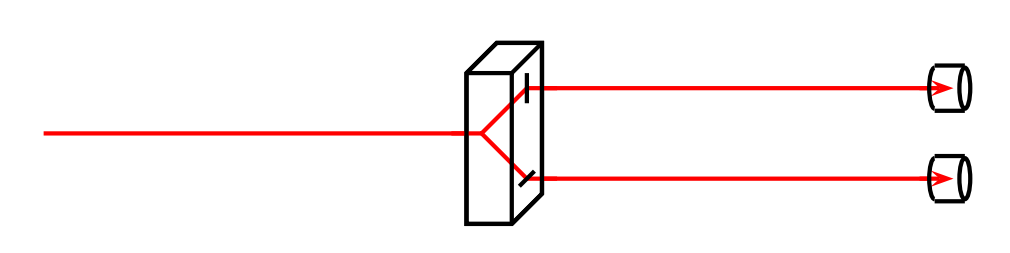
\includegraphics[scale=0.5]{img/dvolomac_detektor.png}
\caption{Dvolomac s dva detektora} 
\end{figure}

Nakon detekcije, foton je apsorbiran i ne može se više mjeriti. Takav kvantnomehanički sustav, koji je moguće samo jednom izmjeriti u samo jednom od dva moguća stanja naziva se \textbf{kvantnim bitom} ili \textbf{qubitom}.
Kvantni bit prije mjerenja može biti u beskonačno mnogo različitih stanja te se općenito jedno takvo stanje naziva \textbf{superpozicijom} dvaju stanja. Ta dva stanja se odnose na stanja baze mjerenja koja mogu biti proizvoljna, ali su uvijek međusobno ortogonalna. Pojam superpozicije se može primijeniti i u klasičnom smislu. U slučaju svjetlosti, uzimajući dva linearno polarizirana vala s okomitim smjerovima polarizacije kao bazu sustava, općenito stanje polarizacije vala može se prikazati kao:
\begin{equation}
E = E_x \hat{x}e^{i(\omega t + \phi_x)} + E_y \hat{y}e^{i(\omega t + \phi_y)} = E_0(\lambda \hat{x} + \mu \hat{y})e^{i\omega t}
\end{equation}
gdje vrijedi:
\begin{equation}
E_0 = \sqrt{(E_x^2 + E_y^2)}
\qquad
\lambda = \frac{E_x}{E_0}e^{i\phi_x}
\qquad
\mu = \frac{E_y}{E_0}e^{i\phi_y}
\qquad
|\lambda|^2 + |\mu|^2 = 1
\end{equation}
Bitno je uočiti da su $\lambda$ i $\mu$ kompleksni brojevi kao i da dio izraza $\lambda\hat{x}+\mu\hat{y}$ sadrži informaciju o stanju polarizacije vala te da takvih stanja ima beskonačno mnogo.

\subsection{Diracova notacija}
Stanja kvantnih bitova u praksi se prikazuje \textit{ket} simbolima koji su dio Diracove ili \textit{bra-ket} notacije:
%\begin{equation} 
\[
\text{\textit{bra}:}
\qquad
\bra{\Phi}
\]
%\end{equation}
%\begin{equation}
\[
\text{\textit{ket}:}
\qquad
\ket{\Phi}
\]
%\end{equation}
%\begin{equation}
\[
\text{\textit{braket}:}
\qquad
\braket{\Phi|\Phi}
\]
%\end{equation}
S pretpostavkom da su $\ket{x}$ i $\ket{y}$ dva stanja baze mjerenja sustava, kao npr. stanje fotona polariziranog u smjeru $x$ i stanje fotona polariziranog u smjeru $y$, općenito stanje polarizacije fotona može se prikazati superpozicijom ta dva stanja:
\begin{equation}
\ket{\Phi} = \lambda\ket{x} + \mu\ket{y}
\end{equation}
gdje su $\lambda$ i $\mu$ kompleksni brojevi te vrijedi $|\lambda|^2 + |\mu|^2 = 1$.

\subsection{Svojstva Hilbertovog prostora}
U matematičkom smislu, stanja kvantnih bitova prikazanih \textit{ketovima} su zapravo vektori dvodimenzionalnog kompleksnog Hilbertovog prostora. Za takav prostor vrijede sljedeća svojstva.

Skalarni umnožak:
\begin{equation}
\braket{\Phi|\Psi} = \braket{\Psi|\Phi}^* \in \mathbb{C}
\end{equation}
\begin{equation}
\braket{\Phi|\Phi} \geq 0
\end{equation}

Norma vektora $\ket{\Phi}:$
\begin{equation}
||\Phi|| = \sqrt{\braket{\Phi|\Phi}}
\end{equation}

Vektori stanja baze moraju biti ortonormirani što znači da mora vrijediti:
\begin{equation}
\braket{x|y} = 0
\qquad
\braket{x|x} = \braket{y|y} = 1
\end{equation}

Za računanje skalarnog umnoška potrebno je izračunati \textit{bra} nekog stanja koji se dobiva kompleksnom konjugacijom \textit{keta}. Općenito, izračun $\braket{\Psi|\Phi}$ dobiva se:
\begin{align*}
\ket{\Phi} &= \lambda\ket{x} + \mu\ket{y} \\
\ket{\Psi} &= \nu\ket{x} + \sigma\ket{y} \Rightarrow \bra{\Psi} = \nu^*\bra{x} + \sigma^*\bra{y} \\
\braket{\Psi|\Phi} &= \nu^*\lambda\braket{x|x} + \nu^*\mu\braket{x|y} + \sigma^*\lambda\braket{y|x} + \sigma^*\mu\braket{y|y} = \nu^*\lambda + \sigma^*\mu = \braket{\Phi|\Psi}^*
\end{align*}
Norma vektora se računa na analogan način.

\subsection{Amplituda vjerojatnosti i vjerojatnost}

Amplituda vjerojatnosti modelira prijelaz jednog kvantnog stanja u drugo koji se računa skalarnim umnoškom vektora stanja.
\begin{equation}
a(\Phi \rightarrow \Psi) = \braket{\Psi|\Phi}
\end{equation}
Odgovarajuća vjerojatnost mjerenja kvantnog bita u stanju $\Psi$ ako se prethodno nalazio u stanju $\Phi$ računa se:
\begin{equation}
p(\Phi \rightarrow \Psi) = |a(\Phi \rightarrow \Psi)|^2 = |\braket{\Psi|\Phi}|^2
\end{equation}

\subsection{Vektorski prikaz}

Za lakšu implementaciju kvantnog bita na klasičnom računalu, korisno je prikazati kvantne bitove vektorski. Klasična nula i jedinica bi imale vektorski oblik:
\begin{equation}
0 = \begin{bmatrix}
1 \\ 0
\end{bmatrix}
\qquad
1 = \begin{bmatrix}
0 \\ 1
\end{bmatrix}
\end{equation}
Ti vektori odgovaraju ujedno i vektorima stanja baze mjerenja nekog sustava koji se mogu označiti kao $\ket{0}$ i $\ket{1}$. Sva ostala stanja mogu se dobiti superpozicijom tih vektora:
\begin{equation}
\ket{\Phi} = \lambda\ket{0} + \mu\ket{1} = \lambda\begin{bmatrix}
1 \\ 0
\end{bmatrix} + \mu\begin{bmatrix}
0 \\ 1
\end{bmatrix} = \begin{bmatrix}
\lambda \\ \mu
\end{bmatrix}
\end{equation}
\textit{Bra} se dobiva kompleksnim konjugiranjem i transponiranjem \textit{keta}:
\begin{equation}
\bra{\Psi} = \begin{bmatrix}
\nu \\ \sigma
\end{bmatrix}^\dagger
= \begin{bmatrix}
\nu^* & \sigma^*
\end{bmatrix}
\end{equation}
Računanje amplitude vjerojatnosti se tada svodi na jednostavno matrično množenje:
\begin{equation}
\braket{\Psi|\Phi} = \begin{bmatrix}
\nu^* & \sigma^*
\end{bmatrix}
\begin{bmatrix}
\lambda \\ \mu
\end{bmatrix} = \nu^*\lambda + \sigma^*\mu
\end{equation}



\section{Sustav kvantnih bitova}

\subsection{Dva ili više kvantnih bitova}
Kao što se jedan kvantni bit prikazuje kao vektor u dvodimenzionalnom kompleksnom Hilbertovom prostoru, sustav od $n$ kvantnih bitova može se prikazati kao vektor u $2^n$-dimenzionalnom kompleksnom Hilbertovom prostoru.

Za $n$ stanja oblika $\ket{\Phi_i},i \in \{1, 2, \ldots, n\}$, njihov zajednički vektor stanja $\ket{\Psi}$ dobiva se \textbf{tenzorskim produktom} svih stanja:
\begin{equation}
\ket{\Psi} = \ket{\Phi_1} \otimes \ket{\Phi_2} \otimes \ldots \otimes \ket{\Phi_n}
\end{equation}

Za dva kvantna bita, tenzorski produkti vektora stanja baze mjerenja sustava označavaju se kao:
\begin{equation}
\ket{0} \otimes \ket{0} = \ket{00} \qquad  \ket{0} \otimes \ket{1} = \ket{01} \qquad \ket{1} \otimes \ket{0} = \ket{10} \qquad \ket{1} \otimes \ket{1} = \ket{11}
\end{equation}
U vektorskom obliku te baze se prikazuju kao:
\begin{equation}
\ket{00} = \begin{bmatrix}
1 \\ 0 \\ 0 \\ 0
\end{bmatrix}
\qquad
\ket{01} = \begin{bmatrix}
0 \\ 1 \\ 0 \\ 0
\end{bmatrix}
\qquad
\ket{10} = \begin{bmatrix}
0 \\ 0 \\ 1 \\ 0
\end{bmatrix}
\qquad
\ket{11} = \begin{bmatrix}
0 \\ 0 \\ 0 \\ 1
\end{bmatrix}
\end{equation}
Općenito, za dva kvantna bita dana u obliku $\ket{\Phi_i} = \lambda_i\ket{0} + \mu_i\ket{1}, i \in \{1, 2\}$, tenzorski produkt jednak je:
\begin{align}
\begin{split}
\ket{\Phi_1} \otimes \ket{\Phi_2} &= (\lambda_1\ket{0} + \mu_1\ket{1}) \otimes (\lambda_2\ket{0} + \mu_2\ket{1})
\\
&= \lambda_1\lambda_2\ket{00} + \lambda_1\mu_2\ket{01} + \mu_1\lambda_2\ket{10} + \mu_1\mu_2\ket{11}
\label{eq:tensor2qubits}
\end{split}
\end{align}
U vektorskom obliku:
\begin{equation}
\ket{\Phi_1} \otimes \ket{\Phi_2} =
\begin{bmatrix}
\lambda_1 \\ \mu_1
\end{bmatrix}
\otimes
\begin{bmatrix}
\lambda_2 \\ \mu_2
\end{bmatrix}
=
\begin{bmatrix}
\lambda_1
	\begin{bmatrix}
	\lambda_2 \\ \mu_2
	\end{bmatrix} \\
\mu_1
	\begin{bmatrix}
	\lambda_2 \\ \mu_2
	\end{bmatrix}
\end{bmatrix}
=
\begin{bmatrix}
\lambda_1\lambda_2 \\
\lambda_1\mu_2 \\
\mu_1\lambda_2 \\
\mu_1\mu_2 \\
\end{bmatrix}
\end{equation}
Analogno se dobiju vektori 3 ili više kvantnih bitova. Naravno, za svaki vektor koji opisuje sustav od $n$ kvantnih bitova oblika
\begin{equation}
\lambda_1\ket{00 \ldots 00} + \lambda_2\ket{00 \ldots 01} + \ldots + \lambda_{2^n}\ket{11 \ldots 11}
\end{equation}
vrijedi:
\begin{equation}
|\lambda_1|^2 + |\lambda_2|^2 + \ldots + |\lambda_{2^n}|^2 = 1
\label{eq:sumofcoefs}
\end{equation}

\subsection{Spregnutost}

Spregnutost \engl{entanglement} opisuje sustav kvantnih bitova koji se ne može prikazati tenzorskim produktom vektora stanja pojedinih kvantnih bitova. Bitno je uočiti da iz jednadžbe \ref{eq:tensor2qubits} vrijedi da je umnožak koeficijenata uz $\ket{00}$ i $\ket{11}$ jednak umnošku koeficijenata uz $\ket{01}$ i $\ket{10}$.
\begin{equation}
\lambda_1\lambda_2 \cdot \mu_1\mu_2 = \lambda_1\mu_2 \cdot \mu_1\lambda_2
\end{equation}
Stanja u kojima vrijedi prethodna jednadžba nazivaju se separabilnima, te zauzimaju samo podskup Hilbertovog prostora u kojemu se nalaze. Vektori stanja koji ne zadovoljavaju takvu jednakost, uz nužan uvjet da zadovoljavaju jednadžbu \ref{eq:sumofcoefs} nazivaju se spregnutim stanjima. Jedno takvo stanje jest:
\begin{equation}
\ket{\Phi} = \frac{1}{\sqrt{2}}(\ket{00} + \ket{11})
\end{equation}
Mjerenje takvog sustava rezultiralo bi detekcijom stanja $\ket{00}$ ili $\ket{11}$, ali nikada  stanja $\ket{01}$ ili $\ket{10}$. Drugim riječima, mjerenjem samo jednog kvantnog bita u sustavu, odmah je poznata i vrijednost drugoga.

Spregnutost se ne odnosi samo na sustave s dva kvantna bita, analogno se ista logika može primijeniti i na sustave s 3 ili više kvantnih bitova. Primjer jednog spregnutog stanja s tri kvantnih bitova:
\begin{equation}
\ket{\Phi} = \frac{1}{\sqrt{2}}(\ket{000} + \ket{111})
\end{equation}




\section{Kvantni operatori}

\subsection{Svojstva}

Kako bi bilo kakav izračun s kvantnim bitovima bio moguć, potrebno je moći manipulirati s njima. S klasičnim bitovima to rade operatori kao što su AND, OR, XOR i sl. Kvantni operatori su nešto drugačiji. Naime, pošto je jedna od glavnih značajki kvantne mehanike reverzibilnost sustava, kvantni operatori moraju biti \textbf{reverzibilni}, što je od klasičnih operatora samo NOT. Pošto stanja kvantnih bitova moraju uvijek ostati normirana, operatori su također \textbf{unitarni}. Uz unitarnost, kvantni operatori su često i \textbf{hermitski}.

\subsection{Blochova sfera}

Radi lakše interpretacije nekih od operatora, korisno je poznavati reprezentaciju kvantnog bita na Blochovoj sferi. Svako stanje\footnote{Odnosi se na čista stanja \engl{pure states}, ali postoje i takozvana mješovita stanja\engl{mixed states} koja se mogu prikazati točkama unutar sfere, ali takva stanja nisu bitna u sklopu ovog rada} kvantnog bita može se prikazati točkom na površini Blochove sfere.

Ta činjenica se čini zbunjujućom jer svaki kvantni bit u potpunosti određuju dva kompleksna broja što rezultira s četiri stupnja slobode, no uzimajući u obzir da kvantni bit mora biti normiran i da množenje kvantnog bita s faznim faktorom nema nikakvog fizičkog utjecaja na njegovo stanje, dobiju se samo dva stupnja slobode. Na temelju toga, općenito stanje kvantnog bita se može izraziti kao:
\begin{equation}
\ket{\Psi} = e^{-i\frac{\varphi}{2}}\cos\frac{\theta}{2}\ket{0} + e^{i\frac{\varphi}{2}}\sin\frac{\theta}{2}\ket{1}
\end{equation}

\begin{figure}[H]
\centering
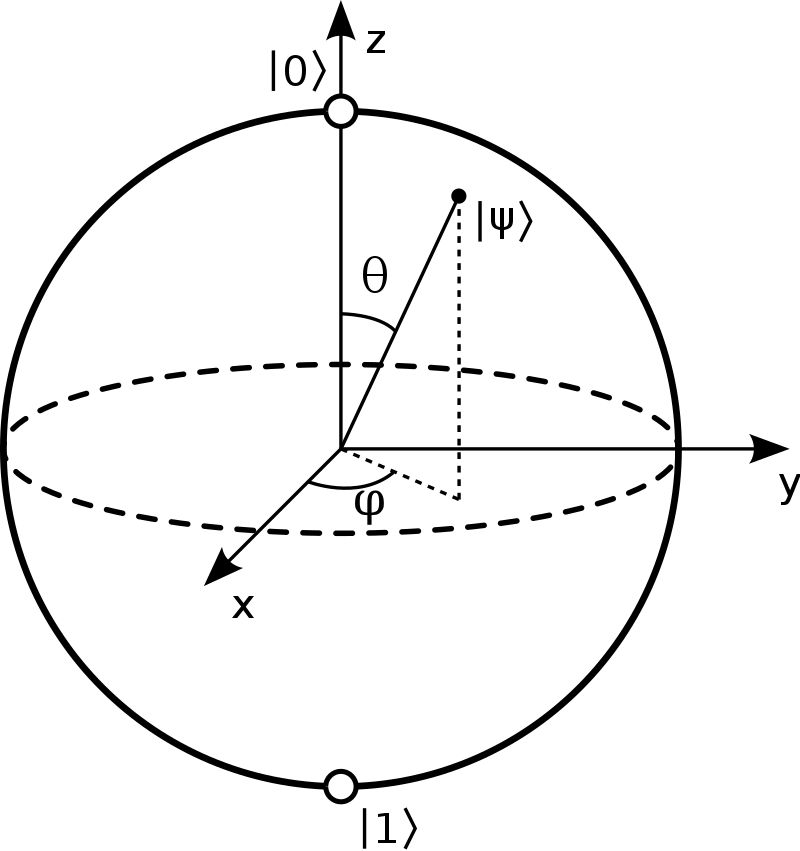
\includegraphics[scale=0.2]{img/bloch.png}
\caption{Blochova sfera} 
\end{figure}

Bitno je primjetiti da vektori koji su u Hilbertovom prostoru ortogonalni su na Blochovoj sferi suprotni. U točki gdje os $x$ probada sferu nalazi se stanje $\frac{1}{\sqrt{2}}(\ket{0} + \ket{1})$, a suprotno njemu $\frac{1}{\sqrt{2}}(\ket{0} - \ket{1})$. Na isti način u smjeru osi $y$ nalazi se stanje $\frac{1}{\sqrt{2}}(\ket{0} + i\ket{1})$ te suprotno njemu $\frac{1}{\sqrt{2}}(\ket{0} - i\ket{1})$. Navedeni vektori označavaju se kao $\ket{x}$ i $\ket{y}$, odnosno $\ket{R}$ i $\ket{L}$.

\subsection{Operator projekcije}

Skalarnim umnoškom dva vektora stanja kvantnih bitova dobije se skalar koji se može interpretirati kao koliko prvi vektor 'ide' u smjeru drugoga. Ako se taj skalar pomnoži drugim vektorom, dobije se vektor projekcije prvoga na drugi.
\begin{equation}
\ket{\Omega} = \ket{\Psi}\braket{\Psi|\Phi}
\end{equation}
Dio izraza $\ket{\Psi}\bra{\Psi}$ možemo shvatiti kao operator projekcije na stanje $\ket{\Psi}$ te se takav operator naziva projektorom. Vektori dobiveni projekcijom općenito nisu normirani te kao takvi ne predstavljaju neko stanje kvantnog bita. Projektori se koriste kako bi se konstruirali drugi operatori.

Matrični prikaz projektora na vektore stanja $\ket{0}$ i $\ket{1}$:
\begin{equation}
\ket{0}\bra{0} =
\begin{bmatrix}
1 \\ 0
\end{bmatrix}
\begin{bmatrix}
1 & 0
\end{bmatrix}
=
\begin{bmatrix}
1 & 0 \\ 0 & 0
\end{bmatrix}
\qquad
\ket{1}\bra{1} = 
\begin{bmatrix}
0 & 0 \\ 0 & 1
\end{bmatrix}
\end{equation}

\subsection{Hermitski operator}

Svaki operator u Hilbertovom prostoru koji je jednak sebi kada se kompleksno konjugira i transponira naziva se Hermitskim operatorom.
\begin{equation}
A^\dagger = A
\end{equation}
Hermitski operator se može prikazati kao linearna kombinacija projektora ortonormirane baze $N$-dimenzionalnog prostora pomnoženih \emph{realnim} koeficijentima:
\begin{equation}
A = \sum_{i = 1}^N a_i\ket{i}\bra{i}
\qquad
a_i \in \mathbb{R}
\end{equation}
Vektori $\ket{i}$ su svojstveni vektori Hermitskog operatora sa odgovarajućim svojstvenim vrijednostima $a_i$.

Hermitski operatori se mogu koristiti za izračune vezane uz fizikalne veličine pripisane baznim stanjima nekog kvantnog sustava, no u sklopu kvantnog računarstva koriste se za manipulaciju stanjima.

\subsection{Paulijeve matrice}

Paulijeve matrice su Hermitske i unitarne matrice koje su često korišteni operatori u kvantnim logičkim krugovima, označavaju se kao X, Y i Z, odnosno $\sigma_x$, $\sigma_y$ i $\sigma_z$. Svojstvene vrijednosti svake Paulijeve matrice su $\pm 1$, dok su svojstveni vektori:
\begin{align}
\sigma_x:&
\qquad
\ket{+} = \frac{1}{\sqrt{2}}(\ket{0} + \ket{1})
\qquad
\ket{-} = \frac{1}{\sqrt{2}}(\ket{0} - \ket{1})
\\
\sigma_y:&
\qquad
\ket{R} = \frac{1}{\sqrt{2}}(\ket{0} + i\ket{1})
\qquad
\ket{L} = \frac{1}{\sqrt{2}}(\ket{0} - i\ket{1})
\\
\sigma_z:&
\qquad
\ket{0}
\qquad
\ket{1}
\end{align}
Njihove vrijednosti iznosee:
\begin{equation}
\sigma_x = \begin{bmatrix}
0 & 1 \\ 1 & 0
\end{bmatrix}
\qquad
\sigma_y = \begin{bmatrix}
0 & -i \\ i & 0
\end{bmatrix}
\qquad
\sigma_x = \begin{bmatrix}
1 & 0 \\ 0 & -1
\end{bmatrix}
\end{equation}
Svaka Paulijeva matrica obavlja operaciju rotacije vektora stanja kvantnog bita za $\pi$ radijana na Blochovoj sferi oko osi po kojoj je nazvana.

Paulijeve matrice su također važne jer linearnom kombinacijom njih i jedinične matrice moguće je konstruirati bilo koji Hermitski operator:
\begin{equation}
A = \lambda_0I + \sum_{i = 1}^3\lambda_i\sigma_i
\label{eq:hermop}
\end{equation}
gdje su svi $\lambda$ koeficijenti realni.


\subsection{Hadamardov operator}

Hadamardov operator obavlja operaciju rotacije od $\pi$ radijana oko osi $\frac{\hat{x} + \hat{z}}{\sqrt{2}}$. Primarno se koristi kako bi se kvantni bit postavio u stanje superpozicije. Njegova vrijednost je:
\begin{equation}
H = \frac{1}{\sqrt{2}}\begin{bmatrix}
1 & 1 \\ 1 & -1
\end{bmatrix}
\end{equation}
Primjer Hadamardovog operatora nad kvantnim bitom $\ket{1}$:
\begin{equation}
H\ket{1} = \frac{1}{\sqrt{2}}\begin{bmatrix}
1 & 1 \\ 1 & -1
\end{bmatrix}
\begin{bmatrix}
0 \\ 1
\end{bmatrix}
= \frac{1}{\sqrt{2}} \begin{bmatrix} 1 \\ -1
\end{bmatrix}
= \begin{bmatrix}
\frac{1}{\sqrt{2}} \\ -\frac{1}{\sqrt{2}}
\end{bmatrix}
\end{equation}
Naravno, zbog reverzibilnosti operatora, ponovnom primjenom Hadamardovog operatora kvantni bit bi se vratio u stanje $\ket{1}$.

\subsection{Ostali unarni operatori}

Svi do sada navedeni operatori djeluju nad samo jednim kvantnim bitom, pa se takvi operatori nazivaju unarnim. Postoje i drugi operatori kao što su $\sqrt{\text{NOT}}$ i operator faznog pomaka $P[\varphi]$:
\begin{equation}
\sqrt{\text{NOT}} = \sqrt{\sigma_x} = \frac{1}{1+i}\begin{bmatrix}
1 & i \\ i & 1
\end{bmatrix}
\qquad
P[\phi] = \begin{bmatrix}
1 & 0 \\ 0 & e^{i\varphi}
\end{bmatrix}
\end{equation}
No, njih kao i sve ostale unitarne Hermitske operatore koje je moguće dobiti na način dan jednadžbom \ref{eq:hermop}, nije potrebno posebno razraditi u sklopu ovoga rada. 

\subsection{CU operatori}

CU operatori ili control-U operatori djeluju na 2 ili više kvantnih bitova od kojih je barem jedan bit \textbf{upravljački}. Općeniti izgled CU operatora za dva kvantna bita u \emph{blok-matričnom} prikazu je:
\begin{equation}
CU = \begin{bmatrix}
I & 0 \\ 0 & U
\end{bmatrix}
\label{eq:cu}
\end{equation}
gdje je $U$ bilo koji unitarni operator, a $I$ jedinična matrica. U načelu, operator provodi operaciju $U$ nad drugim kvantnim bitom ako je prvi u jedinici, inače ga ne mijenja.

Najkorišteniji CU operator jest CX ili CNOT čija se funkcionalnost može opisati kao:
\begin{equation}
CNOT\ket{xy} = \ket{x, y\oplus x}
\end{equation}
gdje je $x$ upravljački bit, a $\oplus$ operator zbrajanja modulo 2. Vrijedi:
\begin{equation}
\begin{aligned}
CNOT\ket{00} = \ket{00} \\
CNOT\ket{01} = \ket{01} \\
CNOT\ket{10} = \ket{11} \\
CNOT\ket{11} = \ket{10}
\end{aligned}
\end{equation}
s odgovarajućom matricom:
\begin{equation}
CNOT = \begin{bmatrix}
I & 0 \\ 0 & \sigma_x
\end{bmatrix} =
\begin{bmatrix}
1 & 0 & 0 & 0 \\ 0 & 1 & 0 & 0 \\ 0 & 0 & 0 & 1 \\ 0 & 0 & 1 & 0
\end{bmatrix}
\end{equation}
Na analogan način se dobiju matrice za CY, CZ i CH unarnih operatora $\sigma_y$, $\sigma_z$, odnosno $H$.

Ovakva konstrukcija CU operatora uvijek pretpostavlja da će prvi kvantni bit biti kontrolni, a onaj nad kojim se vrši operacija drugi. Pošto je na kvantnom računalu moguće da bilo koja dva para kvantnih bitova budu operandi, korisno je, za svrhu izgradnje kvantnog simulatora, na drugačiji način prikazati konstrukciju CU operatora. Sljedeća jednadžba opisuje CU operator već spomenutog oblika \ref{eq:cu}, gdje je prvi bit kontrolni.
\begin{equation}
CU_{1,2} = \ket{0}\bra{0} \otimes I_2 + \ket{1}\bra{1} \otimes U
\end{equation}
Ukoliko je potrebno izgraditi matricu CU operatora gdje je kontrolni bit drugi, a ne prvi, u prethodnoj jednadžbi potrebno je samo promijeniti redoslijed varijabli na način:
\begin{equation}
CU_{2,1} = I_2  \otimes \ket{0}\bra{0} + U \otimes \ket{1}\bra{1}
\end{equation}

%Bez objašnjenja, moguće je simulirati svaki klasični logički krug s ovim operatorima

\subsection{SWAP operator}

SWAP operator zamjenjuje stanja dvaju kvantnih bitova. Moguće ga je dobiti kombinacijom CNOT operatora:
\begin{equation}
\textit{SWAP} = CNOT_{1,2}\cdot CNOT_{2,1}\cdot CNOT_{1,2} = \begin{bmatrix}
1 & 0 & 0 & 0 \\ 0 & 0 & 1 & 0 \\ 0 & 1 & 0 & 0 \\ 0 & 0 & 0 & 1
\end{bmatrix}
\end{equation}

\subsection{Toffolijeva i Fredkinova vrata}

Toffolijeva vrata ili CCNOT operator jest operator koji djeluje na tri kvantna bita od kojih su dva kontrolna. Oba kontrolna bita moraju biti u jedinici kako bi se obavila operacija NOT nad trećim bitom. Matrična forma CCNOT operatora gdje su prvi i drugi bit kontrolni jest:
\begin{equation}
\textit{CCNOT}= \begin{bmatrix}
1 & 0 & 0 & 0 & 0 & 0 & 0 & 0 \\
0 & 1 & 0 & 0 & 0 & 0 & 0 & 0 \\
0 & 0 & 1 & 0 & 0 & 0 & 0 & 0 \\
0 & 0 & 0 & 1 & 0 & 0 & 0 & 0 \\
0 & 0 & 0 & 0 & 1 & 0 & 0 & 0 \\
0 & 0 & 0 & 0 & 0 & 1 & 0 & 0 \\
0 & 0 & 0 & 0 & 0 & 0 & 0 & 1 \\
0 & 0 & 0 & 0 & 0 & 0 & 1 & 0 \\
\end{bmatrix}
\end{equation}
Toffolijeva vrata također imaju svojstvo da je pomoću njih moguće konstruirati bilo koju Booleovu funkciju što rezultira činjenicom da je na kvantnom računalu moguće na reverzibilan način implementirati sve što je moguće i na klasičnom računalu.

Fredkinova vrata ili drugim imenom CSWAP operator radi točno što mu ime sugerira. Ako je kontrolni bit u jedinici, obavi operaciju SWAP nad ostala dva bita, inače ne radi ništa. Njegova matrica jest:
\begin{equation}
\textit{CSWAP} = \begin{bmatrix}
1 & 0 & 0 & 0 & 0 & 0 & 0 & 0 \\
0 & 1 & 0 & 0 & 0 & 0 & 0 & 0 \\
0 & 0 & 1 & 0 & 0 & 0 & 0 & 0 \\
0 & 0 & 0 & 1 & 0 & 0 & 0 & 0 \\
0 & 0 & 0 & 0 & 1 & 0 & 0 & 0 \\
0 & 0 & 0 & 0 & 0 & 0 & 1 & 0 \\
0 & 0 & 0 & 0 & 0 & 1 & 0 & 0 \\
0 & 0 & 0 & 0 & 0 & 0 & 0 & 1 \\
\end{bmatrix}
\end{equation}

\section{Kvantni logički kurg}

\subsection{Topografija logičkog kruga}

Kvantni logički krug sastoji se od kvantnih bitova i kvantnih logičkih vrata kroz koja prolaze određeni kvantni bitovi. Bitovi su reprezentirani kao paralelne linije na koje se s lijeva na desno primjenjuju odgovarajuća logička vrata. Na kraju logičkog kruga vrši se mjerenje\footnote{Po načelu odgođenog mjerenja \engl{Deferred Measurement Principle} odgađanje mjerenja do kraja logičkog kruga ne utječe na raspodjelu vjerojatnosti ishoda, pa se iz tog razloga mjerenje uvijek smješta na kraj, iako je sasvim moguće mjeriti pojedine kvantne bitove kada se zna da više neće prolaziti kroz neka logička vrata.}.
\begin{figure}[H]
\centering
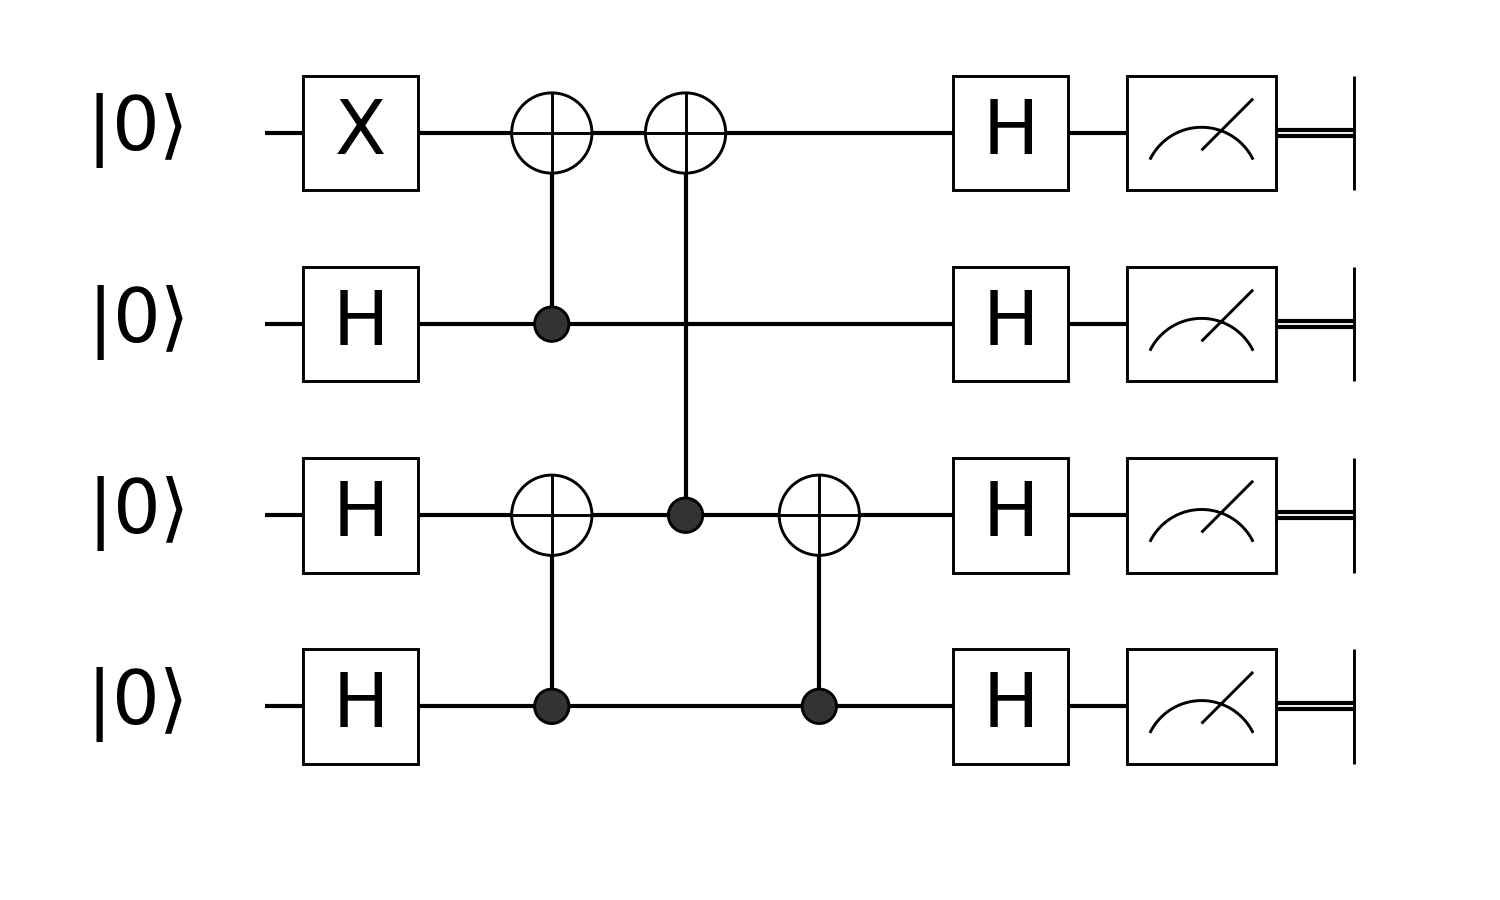
\includegraphics[scale=0.16]{img/exampleqc.png}
\caption{Primjer kvantnog logičkog kruga} 
\end{figure}
Također, standardno je da su svi kvantni bitovi inicijalizirani u stanje $\ket{0}$.

\subsection{Reprezentacija logičkih operatora}

Svaki do sada spomenuti logički operator ima svoju reprezentaciju u kvantnom logičkom krugu. Operatori $\sigma_x$, $\sigma_y$, $\sigma_z$ i Hadamard:
\begin{figure}[H]
\centering
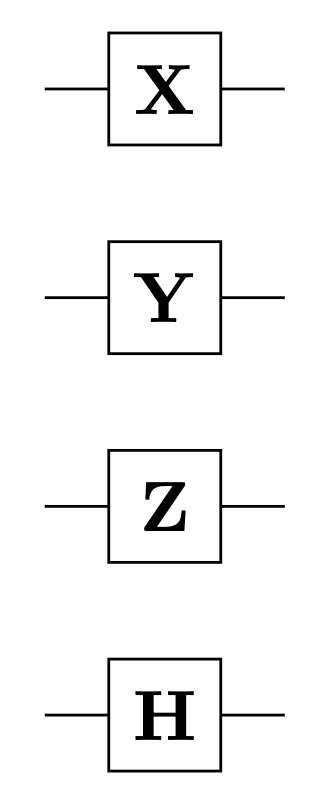
\includegraphics[scale=0.3]{img/xyzh.png}
\caption{Reprezentacija unarnih logičkih operatora} 
\end{figure}
Pošto je $\sigma_x$ često korišten ima i drugi oblik:
\begin{figure}[H]
\centering
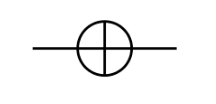
\includegraphics[scale=0.4]{img/xop.png}
\caption{Alternativni $\sigma_x$} 
\end{figure}
CU operatori imaju crnu točku na kontrolnom bitu spojenu vertikalnom crtom sa unarnim operatorom na drugom bitu:
\begin{figure}[H]
\centering
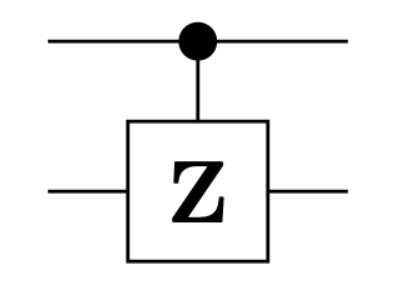
\includegraphics[scale=0.3]{img/CZ.png}
\caption{CZ operator} 
\end{figure}
No, kao i $\sigma_x$, CNOT ima drugačiji prikaz koji se puno češće koristi:
\begin{figure}[H]
\centering
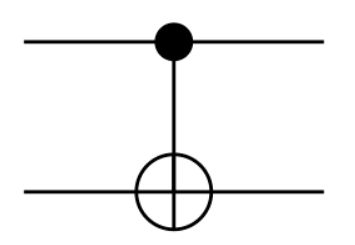
\includegraphics[scale=0.3]{img/CNOT.png}
\caption{CNOT operator} 
\end{figure}
SWAP operator također ima dvije reprezentacije:
\begin{figure}[H]
\centering
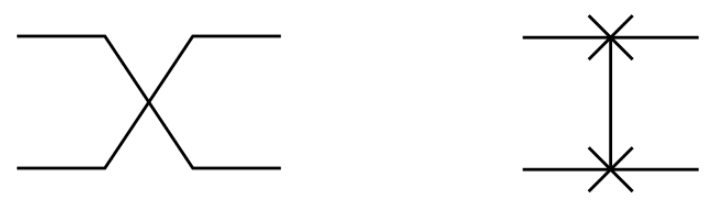
\includegraphics[scale=0.35]{img/SWAP.png}
\caption{SWAP operator} 
\end{figure}
Toffolijeva i Fredkinova vrata:
\begin{figure}[H]
\centering
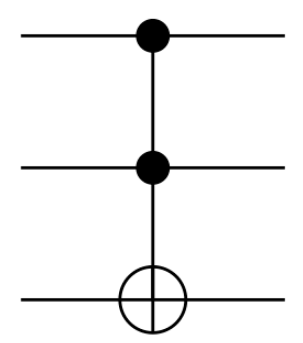
\includegraphics[scale=0.35]{img/CCNOT.png}
\caption{Toffolijeva vrata} 
\end{figure}
\begin{figure}[H]
\centering
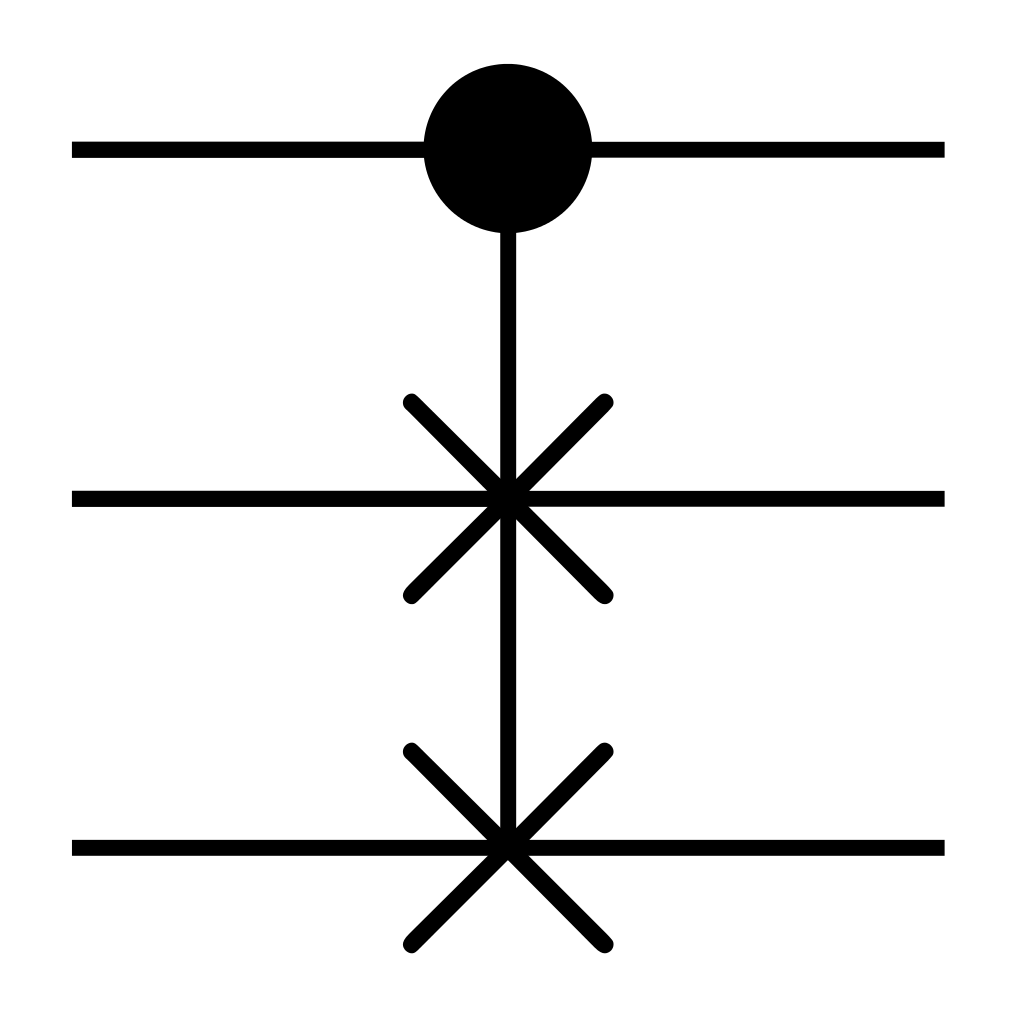
\includegraphics[scale=0.09]{img/CSWAP.png}
\caption{Fredkinova vrata} 
\end{figure}

\subsection{Matrični prikaz}
Svaki kvantni logički krug može se prikazati jednom unitarnom transformacijom. U slučaju kvantnog logičkog kruga s jednim kvantnim bitom, matrica cijelog logičkog kruga dobiva se jednostavnim matričnim množenjem operatora.
\begin{figure}[H]
\centering
\begin{quantikz}
\lstick{$\ket{0}$} & \gate{H} & \gate{Z} & \gate{H} & \qw
\end{quantikz}
\end{figure}
\begin{equation}
U =HZH = \frac{1}{\sqrt{2}} \cdot \frac{1}{\sqrt{2}}
\begin{bmatrix} 1 & 1 \\ 1 & -1  \end{bmatrix}
\begin{bmatrix} 1 & 0 \\ 0 & -1 \end{bmatrix}
\begin{bmatrix} 1 & 1 \\ 1 & -1  \end{bmatrix}
= \frac{1}{2} \begin{bmatrix} 0 & 2 \\ 2 & 0 \end{bmatrix}
= \begin{bmatrix} 0 & 1 \\ 1 & 0 \end{bmatrix}
\end{equation}
Vektor stanja na kraju logičkog kruga:
\begin{equation}
U\ket{0} = \begin{bmatrix}
0 & 1 \\ 1 & 0
\end{bmatrix}
\begin{bmatrix}
1 \\ 0
\end{bmatrix}
= \begin{bmatrix}
0 \\ 1
\end{bmatrix}
= \ket{1}
\end{equation}

Matrica nezavisnih paralelnih operatora dobiva se \emph{tenzorskim produktom} pojedinih operatora, odnosno matricom identiteta ako nema operatora.
\begin{figure}[H]
\centering
\begin{quantikz}
\lstick{$\ket{0}$} & \gate{H} & \qw \\
\lstick{$\ket{0}$} & \qw & \qw \\
\lstick{$\ket{0}$} & \gate{H} & \qw
\end{quantikz}
\end{figure}

\begin{equation}
\begin{aligned}
U = H \otimes I \otimes H &= \frac{1}{\sqrt{2}} \cdot \frac{1}{\sqrt{2}}
\begin{bmatrix} 1 & 1 \\ 1 & -1 \end{bmatrix} \otimes
\begin{bmatrix} 1 & 0 \\ 0 & 1 \end{bmatrix} \otimes
\begin{bmatrix} 1 & 1 \\ 1 & -1 \end{bmatrix} \\
&= \frac{1}{2}
\begin{bmatrix} I & I \\ I & -I \end{bmatrix} \otimes
\begin{bmatrix} 1 & 1 \\ 1 & -1 \end{bmatrix} \\
&= \frac{1}{\sqrt{2}} \begin{bmatrix} H & 0 & H & 0 \\ 0 & H & 0 & H \\ H & 0 & -H & 0 \\ 0 & H & 0 & -H \end{bmatrix}
\end{aligned}
\end{equation}
Stanje sustava na kraju logičkog kruga je:
\begin{equation}
U\ket{000} = \frac{1}{2}
\begin{bmatrix}
1 & 1 & 0 & 0 & 1 & 1 & 0 & 0 \\
1 & -1 & 0 & 0 & 1 & -1 & 0 & 0 \\
0 & 0 & 1 & 1 & 0 & 0 & 1 & 1 \\
0 & 0 & 1 & -1 & 0 & 0 & 1 & -1 \\
1 & 1 & 0 & 0 & -1 & -1 & 0 & 0 \\
1 & -1 & 0 & 0 & -1 & 1 & 0 & 0 \\
0 & 0 & 1 & 1 & 0 & 0 & -1 & -1 \\
0 & 0 & 1 & -1 & 0 & 0 & -1 & 1
\end{bmatrix}
\begin{bmatrix}
1 \\ 0 \\ 0 \\ 0 \\ 0 \\ 0 \\ 0 \\ 0 
\end{bmatrix}
= \begin{bmatrix}
\frac{1}{2} \\ \frac{1}{2} \\ 0 \\ 0 \\ \frac{1}{2} \\ \frac{1}{2} \\ 0 \\ 0 
\end{bmatrix}
\end{equation}
Bitovi 0 i 2 su postavljeni u stanje superpozicije dok je bit 1 ostao u stanju $\ket{0}$ rezultirajući da se mjerenjem sustava uvijek dobije stanje koje na drugom bitu ima nulu. Iz vektora se vidi da se mjerenjem mogu dobiti samo stanja $\ket{000}$, $\ket{001}$, $\ket{100}$ i $\ket{101}$ što odgovara očekivanjima.

Kombinirajući tenzorski produkt i matrično množenje može se izračunati matrična reprezentacija svakog kvantnog logičkog kruga što je u suštini točno ono što izrađeni simulator kvantnog računala i radi.



